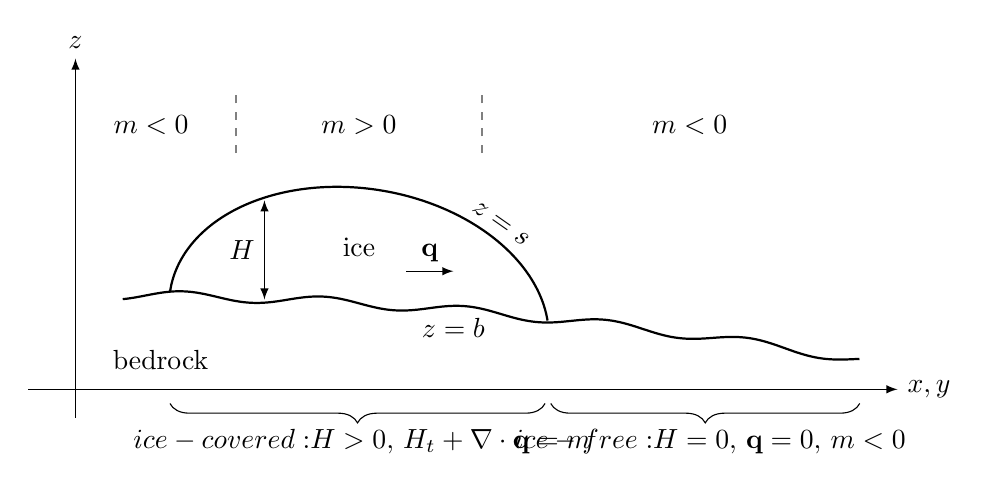
\begin{tikzpicture}[scale=1.2,
declare function={ bed(\x) = 1.0 - 0.01*\x*\x - 0.05*sin(240.0*\x);
                   ice(\x) = 0.7 * sqrt((\x-0.99)*(5.01-\x)) + bed(1.0) - (bed(5.0)-bed(1.0)) * (5.0-\x)/4.0; }]

  % draw axes
  \draw[-latex] (-0.5,0.0) -- (8.7,0.0) node[xshift=4mm] {$x,y$};
  \draw[-latex] (0.0,-0.3) -- (0.0,3.5) node[yshift=2mm] {$z$};

  % bed
  \draw[domain=0.5:8.3,samples=201,variable=\x,black,thick] plot ({\x},{bed(\x)});
  \node at (0.9,0.31) {bedrock};

  % ice surface
  \draw[domain=1.0:5.0,samples=301,variable=\x,black,thick] plot ({\x},{ice(\x)-0.47});  % down-shift needed to fix; WHY?

  % labels/arrows on or within ice
  \node at (3.0,1.5) {ice};
  \node[rotate=-35] at (4.5,1.75) {$z=s$};
  \node at (4.0,0.65) {$z=b$};
  \draw[-latex] (3.5,1.25) -- (4.0,1.25) node[midway,above] {$\mathbf{q}$};
  \draw[latex-latex] (2.0,0.95) -- (2.0,2.0) node[midway,left] {$H$};

  % labels and dashed lines showing CMB zones
  \node at (0.8,2.8) {$m<0$};
  \draw[dashed,thick,gray] (1.7,2.5) -- (1.7,3.2);
  \node at (3.0,2.8) {$m>0$};
  \draw[dashed,thick,gray] (4.3,2.5) -- (4.3,3.2);
  \node at (6.5,2.8) {$m<0$};

  % underbraces with labels
  \draw[decorate,decoration={brace,amplitude=7pt,mirror}] (1.0,-0.15) -- (4.97,-0.15) node[below,midway,yshift=-2mm] {$\begin{matrix} \text{ice-covered:} \\ H>0, \, H_t+\nabla\cdot\mathbf{q}=m \end{matrix}$};
  \draw[decorate,decoration={brace,amplitude=7pt,mirror}] (5.03,-0.15) -- (8.3,-0.15) node[below,midway,yshift=-2mm] {$\begin{matrix} \text{ice-free:} \\ H=0, \, \mathbf{q}=0, \, m < 0 \end{matrix}$};

\end{tikzpicture}

